\documentclass[tikz,border=12pt]{standalone}
% Compile each standalone figure from its example subdirectory.
% Shared visual language for standalone EMT block diagrams.
\usepackage{amsmath}
\usetikzlibrary{arrows.meta,backgrounds,calc,fit,positioning}

\tikzset{
    emt diagram/.style = {>={Stealth[length=2.4mm]}},
    line/.style        = {semithick, rounded corners=6pt},
    block/.style       = {draw, semithick, fill=white,
                          minimum height=1cm, minimum width=2.3cm},
    hblock/.style      = {block, minimum width=2.24cm, minimum height=1.3cm},
    vblock/.style      = {block, minimum width=1.3cm, minimum height=2.24cm},
    sum/.style         = {draw, semithick, fill=white, circle,
                          inner sep=2.6pt},
    signal/.style      = {circle, fill, inner sep=1.4pt,
                          label distance=3pt},
    sig/.style         = {font=\small},
    pm/.style          = {font=\scriptsize},
    wire jump/.style   = {line,
                          preaction={draw=white, line width=3pt,
                                     line cap=round}},
    enclosure/.style   = {draw, dashed, semithick, rounded corners=4pt},
    operator enclosure/.style = {enclosure, inner xsep=7mm, inner ysep=6mm}
}


\definecolor{externalBusBlue}{HTML}{007AFF}
\definecolor{internalBusRed}{HTML}{D64545}

\tikzset{
    partition/.style = {enclosure, solid},
    partition group/.style = {enclosure},
    external reference/.style = {line, dashed, draw=black},
    physical branch/.style = {line, solid, draw=black!45},
    external bus/.style = {signal, fill=externalBusBlue},
    internal bus/.style = {signal, fill=internalBusRed},
    external bus label/.style = {sig, text=externalBusBlue, fill=white, inner sep=1pt},
    internal bus label/.style = {sig, text=internalBusRed},
    partition label/.style = {sig, fill=white, inner sep=2pt}
}


% Membership diagram for shared.partition.json.
% Connectors identify copies of the same external bus, not electrical branches.
% TUNABLES: scale the complete figure; coordinates below remain editable.
\def\diagramScale{1}

\begin{document}
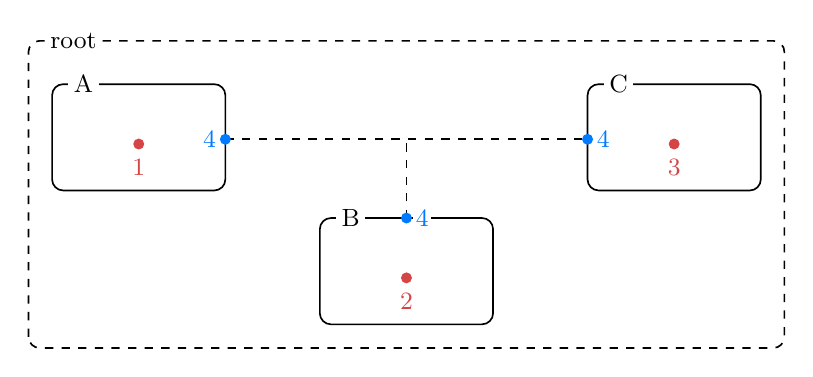
\begin{tikzpicture}[emt diagram, scale=\diagramScale, transform shape]

% Group enclosures are organizational only.
\draw[partition group] (-1.4, -2.65) rectangle (8.2, 1.25);
\node[partition label, anchor=west] at (-1.2, 1.25) {root};

% Leaf partitions.
\draw[partition] (-1.1, -0.65) rectangle (1.1, 0.7);
\node[partition label, anchor=west] at (-0.9, 0.7) {A};
\draw[partition] (2.3, -2.35) rectangle (4.5, -1.0);
\node[partition label, anchor=west] at (2.5, -1.0) {B};
\draw[partition] (5.7, -0.65) rectangle (7.9, 0.7);
\node[partition label, anchor=west] at (5.9, 0.7) {C};

% Black lines join border copies of the same external bus.
% Bus 4: A <-> C, with B joining the same connector.
\draw[external reference] (1.1, 0) -- (5.7, 0);
% Bus 4: B joins A and C.
\draw[external reference] (3.4, -1.0) -- (3.4, 0);

% Internal buses appear only inside their owning leaf.
\node[internal bus, label={[internal bus label]below:$1$}] (bus1) at (0, -0.06) {};
\node[internal bus, label={[internal bus label]below:$2$}] (bus2) at (3.4, -1.76) {};
\node[internal bus, label={[internal bus label]below:$3$}] (bus3) at (6.8, -0.06) {};

% Each external bus has one copy on every referencing Partition border.
% A references bus 4.
\node[external bus, label={[external bus label]left:$4$}] (bus4-A) at (1.1, 0) {};
% B references bus 4.
\node[external bus, label={[external bus label]right:$4$}] (bus4-B) at (3.4, -1.0) {};
% C references bus 4.
\node[external bus, label={[external bus label]right:$4$}] (bus4-C) at (5.7, 0) {};

\end{tikzpicture}
\end{document}
